\section{Work Breakdown Structure}

\begin{figure}[H]
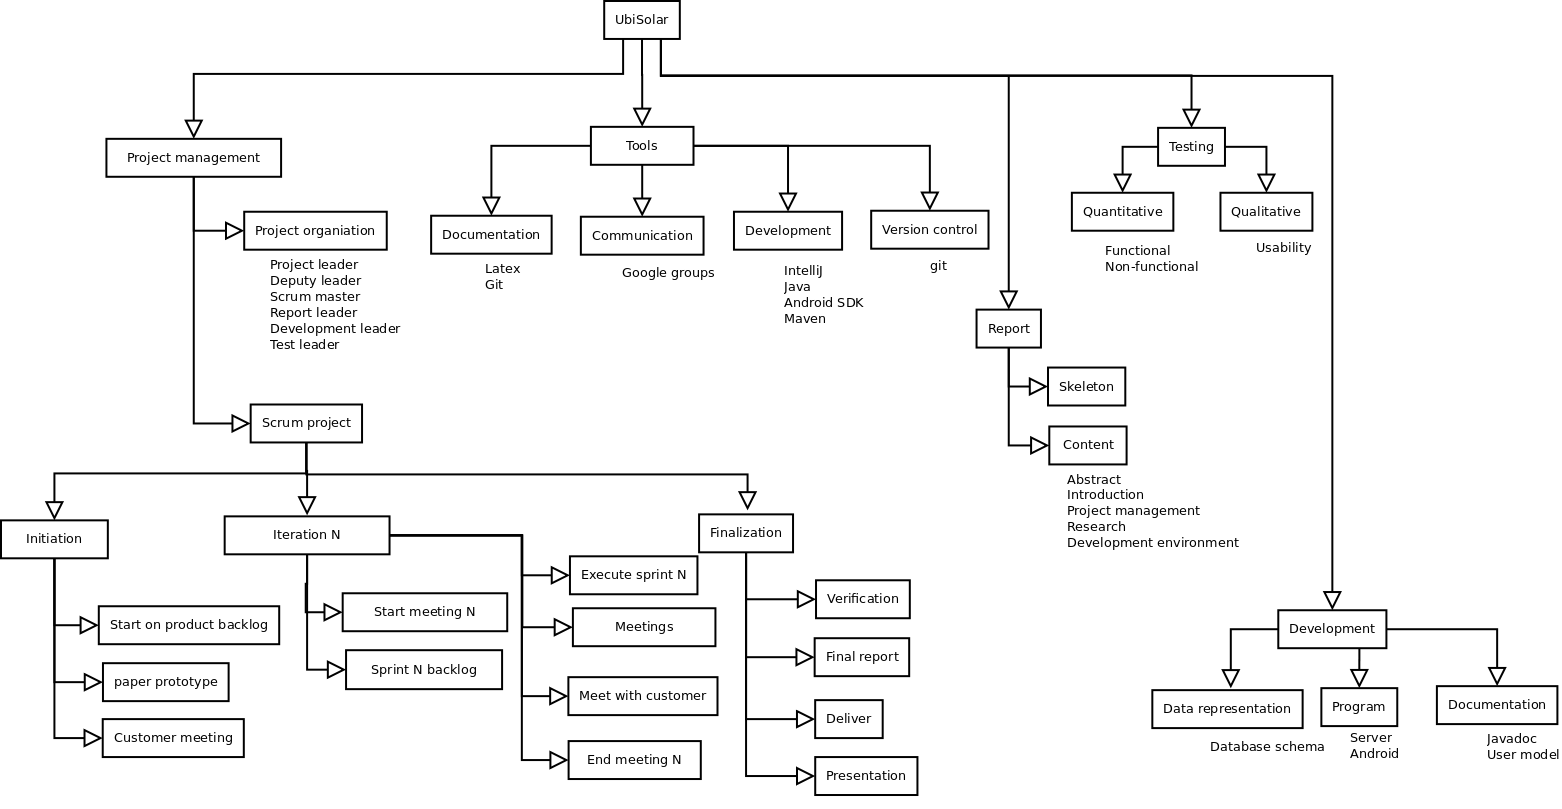
\includegraphics[width=\textwidth]{ch/projectPlan/fig/WBS.png}
\caption{The work breakdown structure}
\todo[inline]{Skal det være produktorientert eller rette seg mot hele prosjektet? Dette må gjenspeiles i caption}
\end{figure}

The work breakdown structure is broken down into five parts. Each part is a package that represents a part of the work that needs to be done in the project.
The reason for using WBS is so that the team can analyze of much time that is actually spent on the different parts of the project compared to how it was planned.
The effect of doing this is that one can easily see if some part of the project gets forgotten or gets too much time.

\missingfigure{Add figure meta data}
\todo[inline]{add hours}
\begin{table}[H]
\centering
\rowcolors{1}{darkgray}{lightgray}
\begin{tabular}{l c r}
    \textbf{WB \#} & \textbf{Name} & \textbf{Hours} \\\hline
    1 & Project management & \\\hline
    2 & Tools & \\\hline
    3 & Report & \\\hline
    4 & Development & \\\hline
    5 & Testing  & \\\hline
\end{tabular}
\end{table}

The team has set aside a certain amount of time to each work breakdown package.
